\documentclass{article}
\usepackage{tikz} 
\usepackage[utf8]{inputenc}
\usepackage{amsmath}
\usepackage{listings}
\usepackage{amsfonts}
\usepackage{amssymb}
\usepackage{tabularx}
\usepackage{enumitem}
\usepackage{algorithm}% http://ctan.org/pkg/algorithm
\usepackage[noend]{algpseudocode}% http://ctan.org/pkg/algorithmicx

\usepackage{tikz}

\usepackage{graphicx}
\usetikzlibrary{arrows,positioning} 
\usepackage{subcaption}
\thispagestyle{empty}
\usepackage{multicol,caption}
\pgfarrowsdeclarecombine{ring}{ring}{}{}{o}{o}

\DeclareMathOperator{\ringarrow}{\raisebox{0.5ex}{\tikz[baseline]{\draw[ring->](0,0)--(2em,0);}}}

\tikzset{
    %Define standard arrow tip
    >=stealth',
    %Define style for boxes
    observed/.style={
           circle,
           rounded corners,
           draw=black, thick,
           minimum width=1em,
           minimum height=1em,
           font=\footnotesize,
           text centered,
           fill=blue!20!white},
     latent/.style={
           circle,
           rounded corners,
           draw=black, thick, dashed,
           minimum width=.5em,
           minimum height=.5em,
           font=\footnotesize,
           text centered,
           fill=black!10!white
           },
    % Define arrow style
    pil/.style={
           o->,
           thick,
           shorten <=2pt,
           shorten >=2pt,},
    sh/.style={ shade, shading=axis, left color=red, right color=green,
    shading angle=45 }
    
}
   
\begin{document}
\def\ci{\perp\!\!\!\perp} % from Wikipedia


\begin{figure}
\centering
\begin{subfigure}[t]{0.4\textwidth}
\centering
\caption{$G^{\dagger}$}
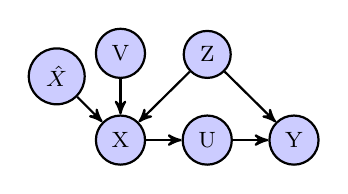
\begin{tikzpicture}[->,shorten >=0pt,shorten <=0pt,node distance=0.45cm,thick,main node/.style={observed}]
\node[main node](1){Z};
\node[main node, below=of 1](2){U};
\node[main node, left=of 2](3){X};
\node[main node, right=of 2](4){Y};
\node[main node, above=of 3](5){V};
\node[main node, above left=of 3](6){$\hat{X}$};

\path[]
	(1) edge (3) edge (4)
	(3) edge (2)
	(5) edge (3)
	(6) edge (3)
	(2) edge (4);
\end{tikzpicture}
\end{subfigure}
\begin{subfigure}[t]{0.3\textwidth}
\centering
\caption{$G_{\overline{X}}$}
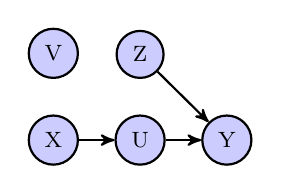
\begin{tikzpicture}[->,shorten >=0pt,shorten <=0pt,node distance=0.45cm,  thick,main node/.style={observed}, shaded/.style={latent}]
\node[main node](1){Z};
\node[main node, below=of 1](2){U};
\node[main node, left=of 2](3){X};
\node[main node, right=of 2](4){Y};
\node[main node, above=of 3](5){V};

\path[]
	(1) edge (4)
	(3) edge (2) 
	(2) edge (4);
	 
\end{tikzpicture}
\end{subfigure}
\end{figure}

\end{document}